\chapter{Ansteuerung des Oszilloskop}
\label{ch:osci}

Im weiteren Verlauf meines Praktikums wurde mir irgendwann die Ansteuerung und die Implementierung eines Oszilloskopes zu Teil. 
Abbildung \ref{fig:lc334am} zeigt das Lecroy LC334AM 500Mhz Oszilloskop, welches über die \ac{gpib} Schnittstelle mit dem Computer kommunizieren kann. Der \ac{gpib} von \ac{ni}\footnote{\url{http://www.ni.com/de-de.html}} ist ein Industriestandard, welcher als \ac{ieee}\footnote{\url{https://www.ieee.org/}} veröffentlicht wurde.

\begin{figure}[H]
	\centering
	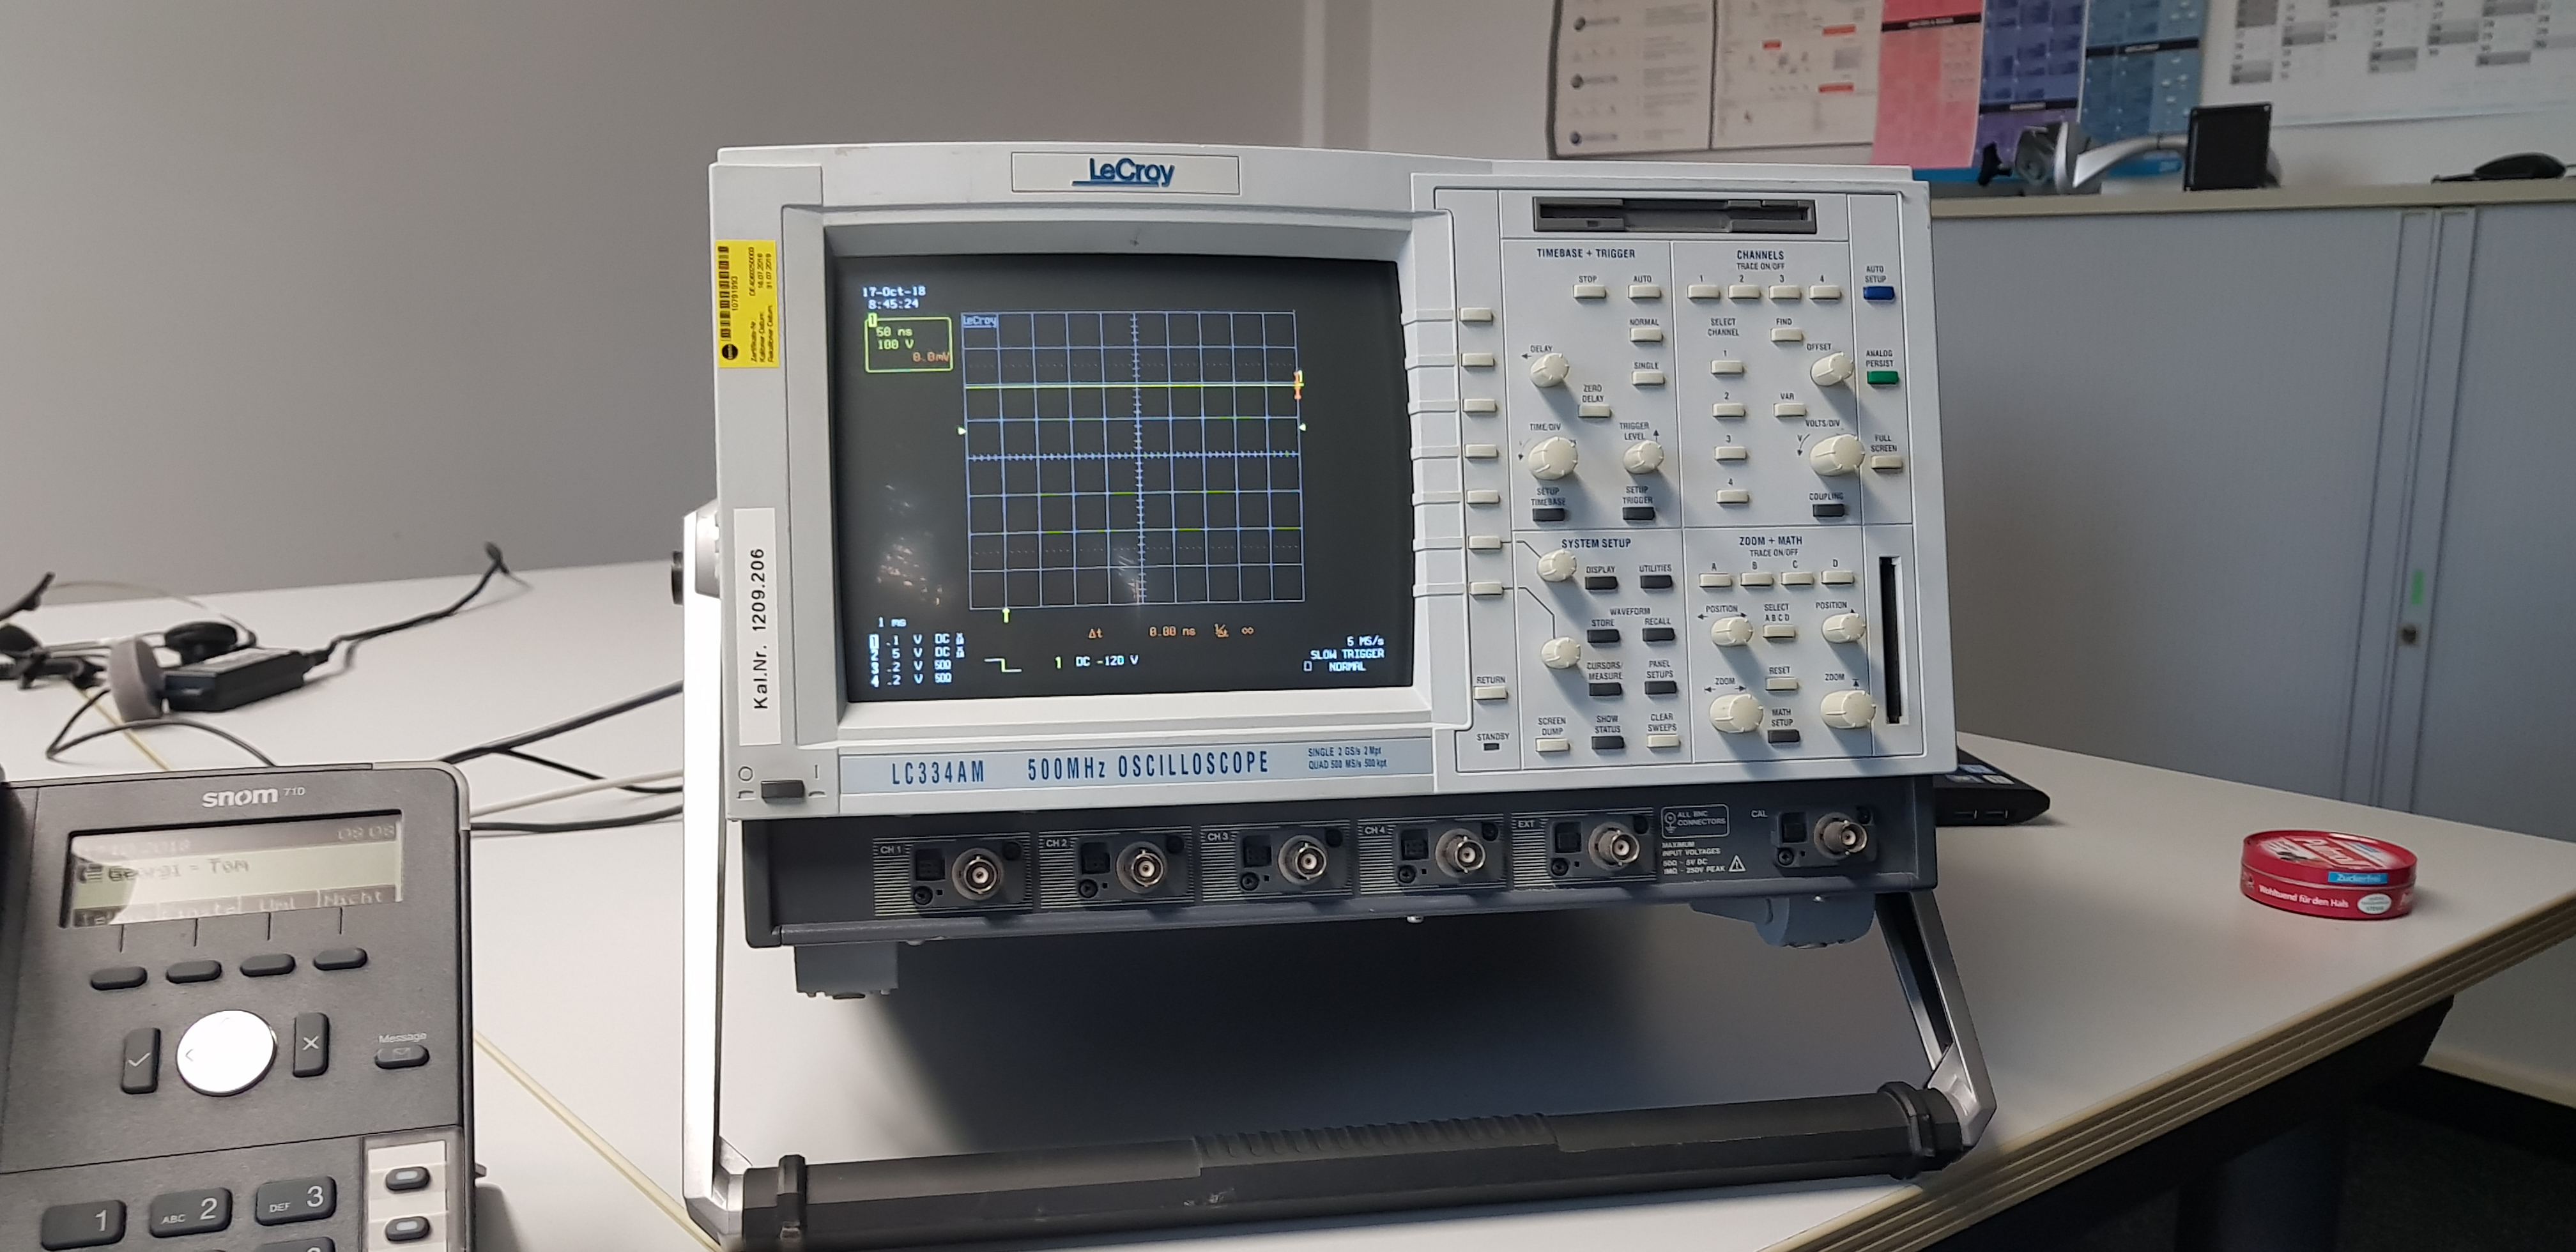
\includegraphics[width=1\textwidth, height=0.5\textwidth]{graphics/Programmed_Oscilloscope.jpg}
	\caption{Lecroy LC334AM 500MHz}
	\label{fig:lc334am}
\end{figure}

